\documentclass[]{assignment}

\begin{document}


%%% INPUT YOUR NAME AND STUDENT NUMBER
%%% INPUT YOUR NAME AND STUDENT NUMBER
%%% --> 13369451
\def\studentname{James Dorrian}
\def\ucdstudentnumber{13369451}
%%% <--
%%% INPUT YOUR NAME AND STUDENT NUMBER
%%% INPUT YOUR NAME AND STUDENT NUMBER


%% HOW TO USE THIS TEMPLATE:
%% No need to keep instruction's text, use this as an template example
%% Replace section content below with your solution
%% Insert Matlab code segments as appropriate
%% Comment and interpret your results 

%% WHAT TO SUBMIT 
%%	1) your pdf report using this latex report
%%	2) an archive of your latex folder
%%  3) your matlab solution in a form of a single commented file


\maketitle

%%%%%%%%%%%%%%%%%%%%%%
%%% 2nd Section
\newpage
\section{{\bf Second Assignment:} Neyman-Pearson Detection}

I built a Neyman-Pearson detector for a known watermark $\mathbf{x}=(x[1],\cdots,x[N])^T$ hidden in a host vector $\mathbf{z}=(z[1],\cdots,z[N])^T$ formed by iid Gaussian variables which are NeymanPearson detectors in Gaussian noise. This assignment consists of a ``Monte Carlo'' simulation (i.e.  using  pseudorandom experiments) of the N-P detector. The second part of the assignment deals with Laplacian distribution. For part 1, I will dicuss my empirical results with the theoretical model below:

%%% First Sub-Section

\subsection{Monte Carlo Simulation}

For the Monte Carlo simulation we generated $1000$ independent and identically distributed pseudorandom vectors with $100$ normally distributed values around a mean of $0$ and a standard deviation of $10$.
\begin{itemize}

\item To compute the threshold values I generated an array called $threshold$ of size 100. Although stated in class that a more simplistic threshold could be used I decided to use the step method which involves increasing the parameter of the Q function by 0.01 each time. We use the q function to create the threshold and steadily increase the distance from the mean a normal (Gaussian) random variable will have to be to operate. We also multiply in the standard deviation and the normalized value of x. This gives us the theoretical probability of false alarm. This is shown in the below code snippet:

\setlength{\fboxsep}{0pt}%
\setlength{\fboxrule}{1pt}%
\fbox{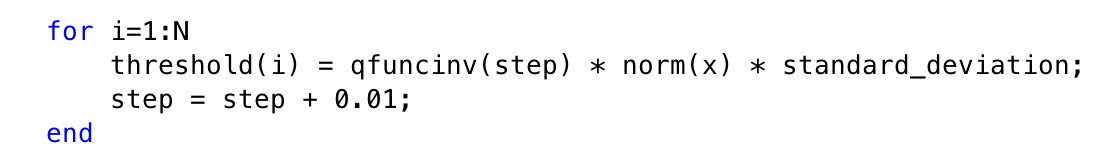
\includegraphics[scale=0.8]{threshold}}


\item I applied the Neyman Pearson test on the 1000 vectors computing the probability of false alarm before the addition of the watermark. This is what we will refer to as out null hypothesis and is used as a control for our experiment. The calculation involves going through each vector, creating 100 normally distributed values and multiplying by the standard deviation. This can be seen in the below code snippet:

\setlength{\fboxsep}{0pt}%
\setlength{\fboxrule}{1pt}%
\fbox{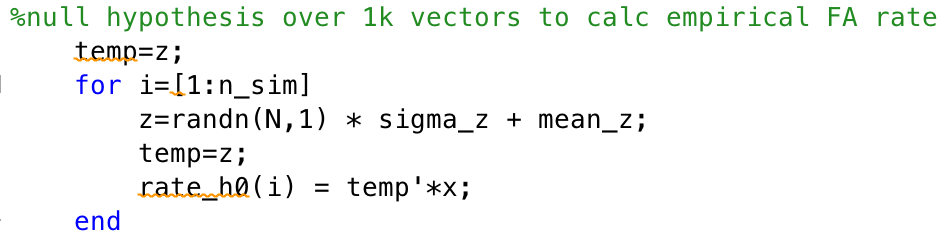
\includegraphics[scale=0.8]{fa_rate}}

\textbf{Note:} temp represents z and temp’ is the transpose of z used for multiplication. This allows for dot product to be calculated.

\item Adding in the watermark denoted as K which will be a watermark of $0.1, 0.5,1$ involves calling our NeymanPearson function 3 times with 3 different parameters: $1, 2, 10$. This watermark is calculated as shown below:


\setlength{\fboxsep}{0pt}%
\setlength{\fboxrule}{1pt}%
\fbox{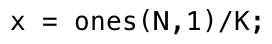
\includegraphics[scale=1]{watermark}}


\item By running the program 3 times at 3 different thresholds, we have achieved 3 empirical ROCs ($P_F^e$ versus $P_D^e$). Below is the plot the empirical results  against the corresponding theoretical ones ($P_F$ versus $P_D$),  using the results given in the lecture. The chance line is plotted in green at the bottom of the image. Observe how the test  improves (better $P_D$ for the same $P_F$) as we increase the level  $K$ of the watermark.


\begin{figure}[h]
\centering
\fboxsep 0mm
\parbox{6cm}{\framebox{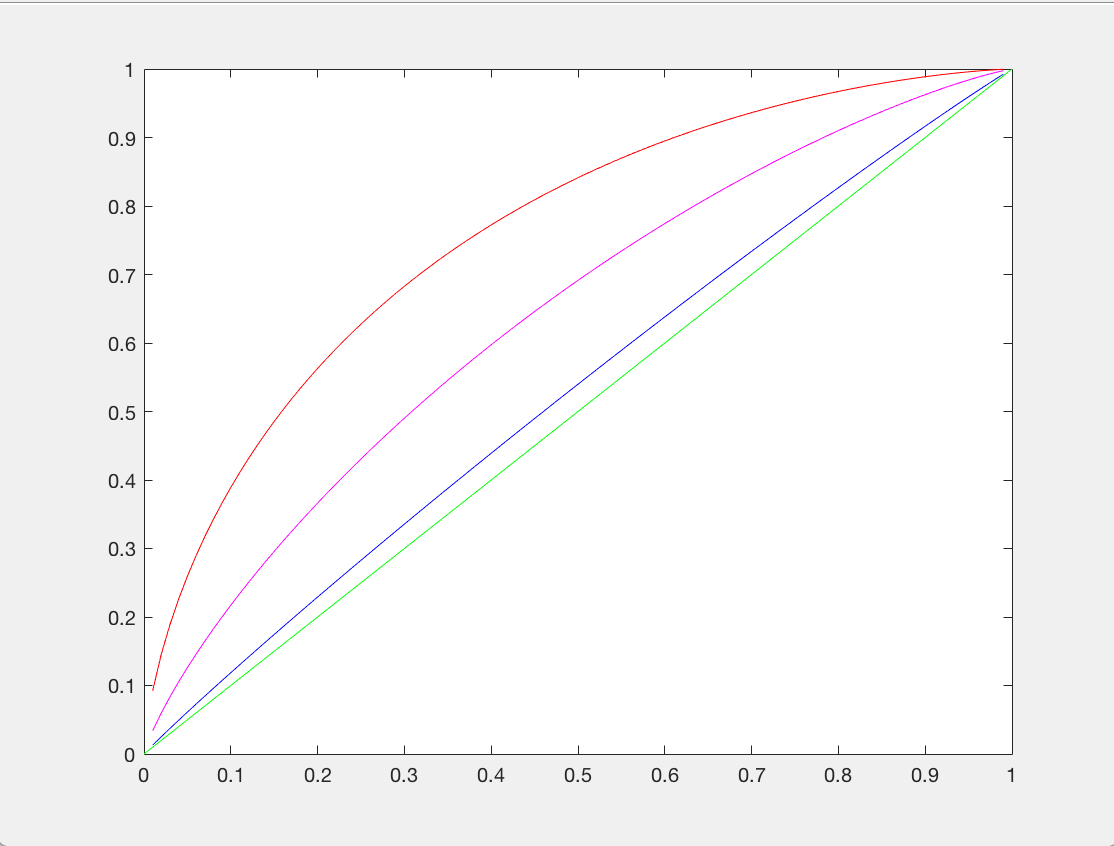
\includegraphics[width=6cm]{theoretical_vals}}\\\centering{(a)}}
~~~
\parbox{6cm}{\framebox{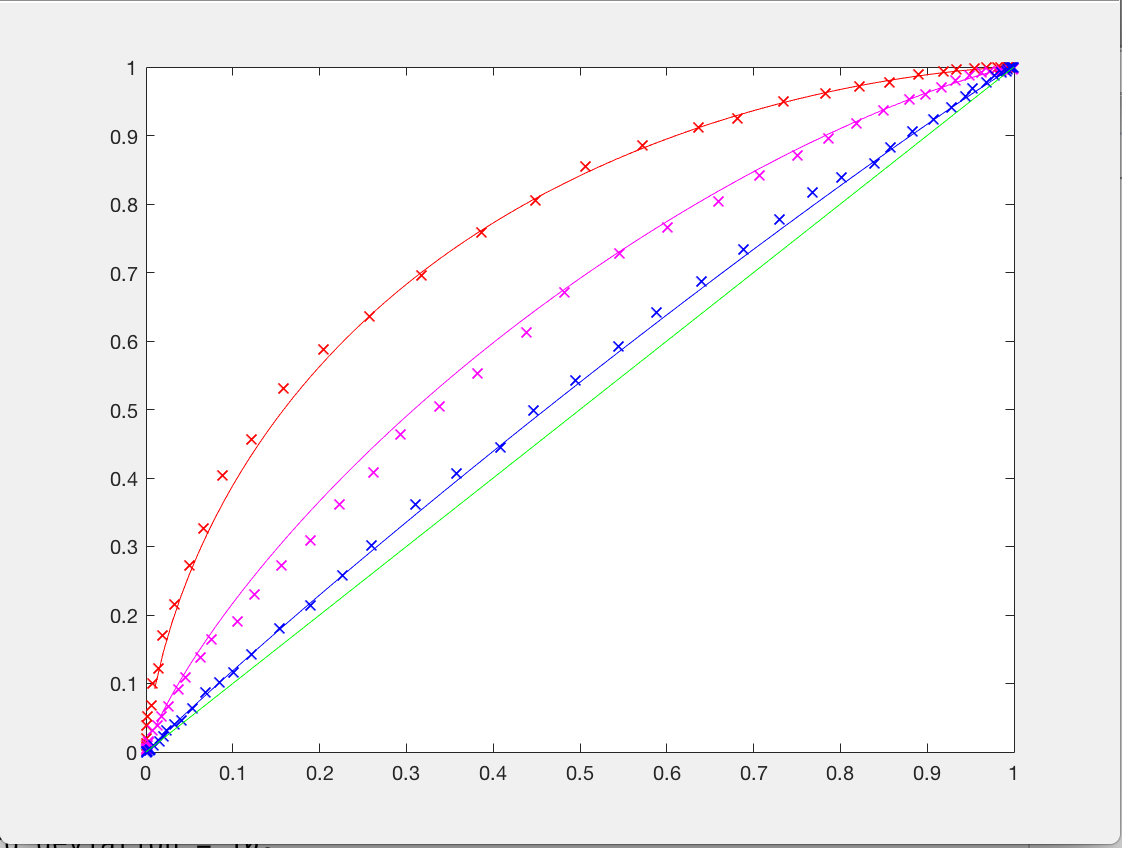
\includegraphics[width=6cm]{results}}\\\centering{(b)}}
\caption{\label{fig:imgfilter1} Theoretical results (a) and empirical results displayed alongside theoretical results (b)}
\end{figure} 

\item Above I have included 2 figures. The x-axis represents the probability of detection and the y-axis represents the false alarm. The first figure contains 4 solid lines, the bottom line is the chance line above that is the first watermarked line with a watermark value of K=0.1, then K=0.5 and finally K=1 are the three lines above.  

\item Both PD and PF are non-decreasing functions, which is evident from figure 1 (b) which shows the ROC for different Gaussian values. This diagram illustrates how the probability of detection and the probability of failure increase but that they do not increase linearly. In continuous likelihood tests like the NP test we are conducting the curve will always have a concave shape. The implication of this is that all values will lie above the chance line and that by seeing how far above the chance line they lie we can determine how well they perform.

\item We used the receiving operator characteristic to plot the difference between PD and PF. It can be seen that where the watermark is highest (K=1.0) performance is best as it is furthest from the chance line. It is interesting to note that where the probability of false alarm is close to 0, so too is the probability of detection. Equally where the probability of false alarm is close to one, so too is the probability of detection. In between, where the probability of false alarm is between 0.2 and 0.6 we see the largest distance of the empirical values from the chance line and therefore the best performance.

\end{itemize}

%%% Second Sub-Section
\clearpage
\subsection{Laplacian Distribution}



For the case where elements of $\mathbf{z}$ are i.i.d. Laplacian, i.e. the pdf of each $z[i]$ for $i=1,\cdots, N$ is in this case: (found as laprnd function in my matlab code)
\[f_Z(z)=\frac{\lambda}{2} \exp(-\lambda|z|),\]

My understanding of question two is as follows: 

\begin{itemize}
\item Instead of having normally distributed values in our vectors, use the laplacian distribution and evaluate how well the results line up. 

\item I graphed my part 1 using the laplacian distribution of vector values. And it produced graph 2(a) but when I multiplied the watermark by the standard deviation it produced 2(b). 

\item As some of the values can be seen to drop below the chance line, I think it is fair to evaluate the laplacian method as a failure. 

\end{itemize}

\begin{figure}[h]
\centering
\fboxsep 0mm
\parbox{6cm}{\framebox{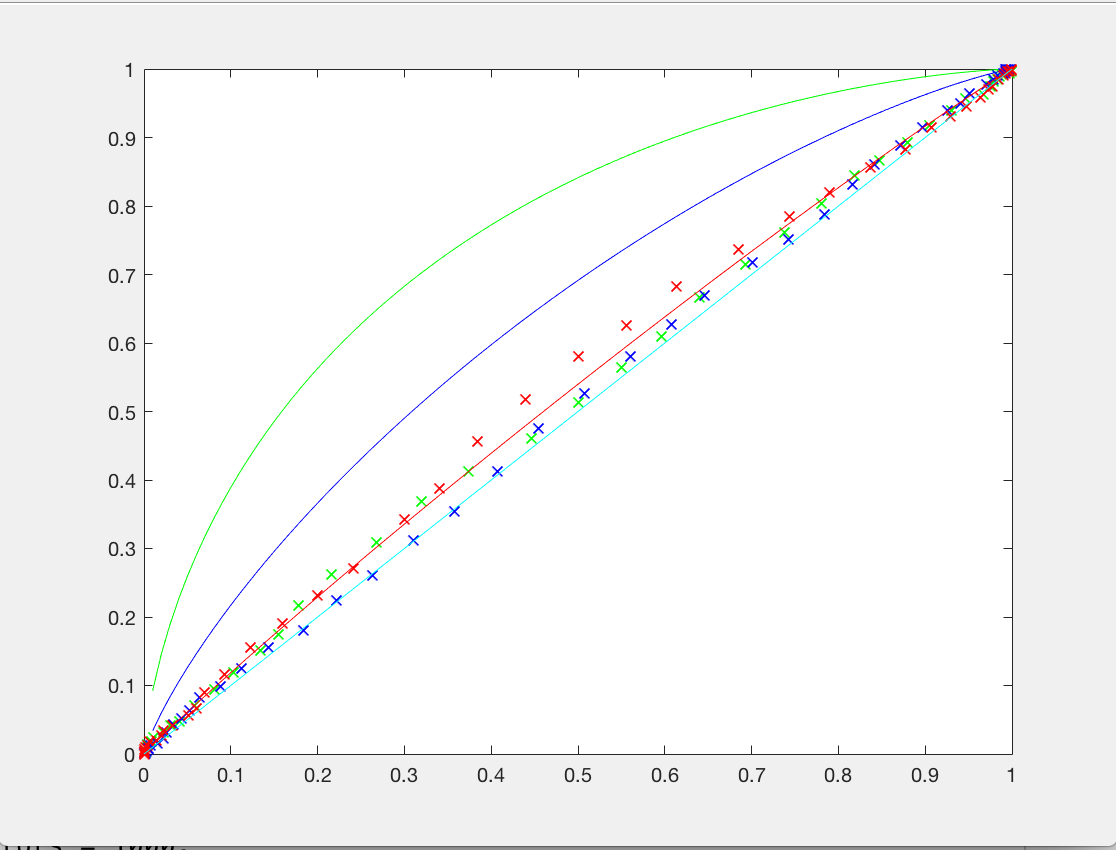
\includegraphics[width=6cm]{fig2a}}\\\centering{(a)}}
~~~
\parbox{6cm}{\framebox{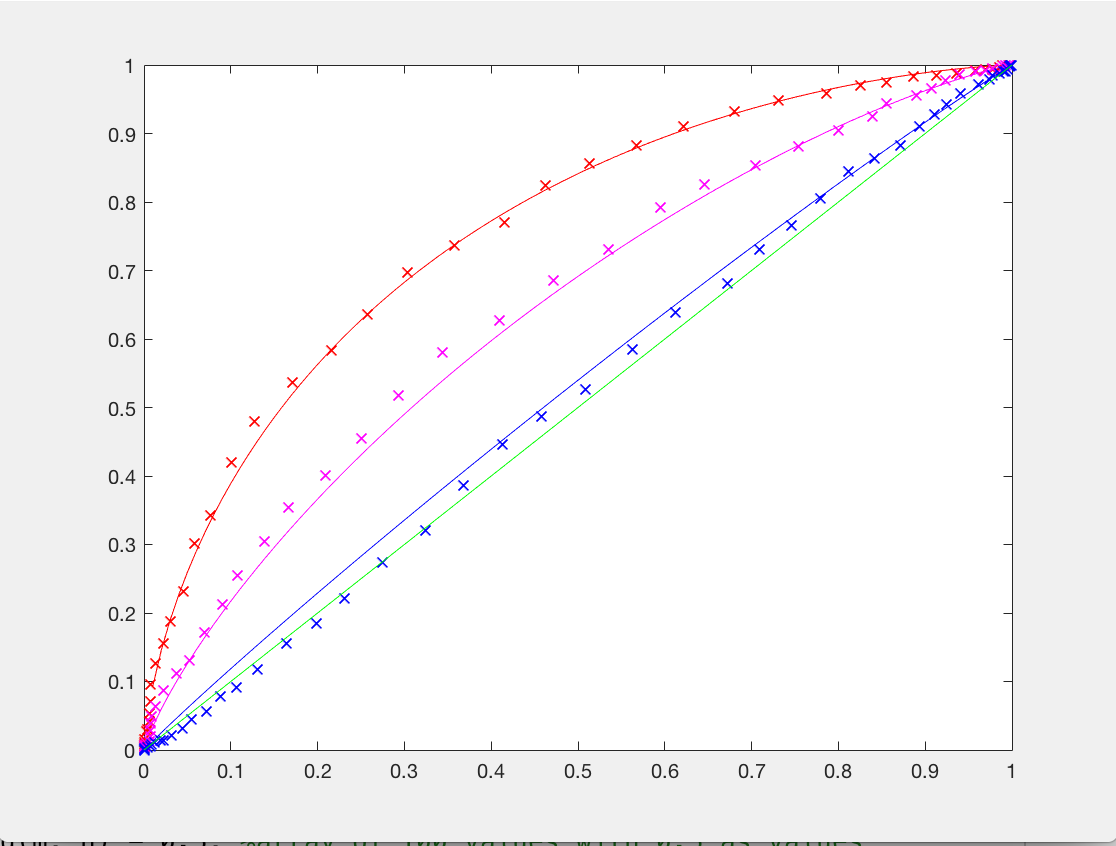
\includegraphics[width=6cm]{fig2b}}\\\centering{(b)}}
\caption{\label{fig:imgfilter1} Theoretical results (a) and empirical results displayed alongside theoretical results (b)}
\end{figure} 
\label{last_page}



%%%%%%%%%%%%%%%%%%%%%%%%%%%%%%%%%%%
%%%%%%%%%%%%%% END %%%%%%%%%%%%%%%%%%
%%%%%%%%%%%%%%%%%%%%%%%%%%%%%%%%%%%


 \end{document} 